\chapter{Discussion}
\label{Discussion}

\section{Dust Disk Characteristics and Stirring Mechanisms}

49 Ceti's unique dust disk and its substantial reservoir of molecular gas given its age are special features that help illuminate the late stages of disk evolution. Its broad dust disk displays a population of small, $\sim$ 0.1\,$\mu m$ grains that extends from $\sim$ 4 to $\sim$ 60\,AU, and a population of larger, $\sim$ 1.6\,$\mu m$ grains that extends from $\sim$ 60 to $\sim$ 300\,AU. The surface density of the dust peaks at $\sim$ 110\,AU, suggesting a region of enhanced collisions between planetesimals. Preliminary analysis of the CO emission suggests that a substantial mass of CO is co-located with the dust, indicating that similar processes may be shaping their morphologies. 

\subsection{Self-Stirring}
\label{SelfStirring}

Replenishment of mm-sized grains through destructive collisions of planetesimals requires impact velocities that can only be achieved in a dynamically stirred environment \citep{Moor13}. Self-stirring scenarios, in which $\sim$ 1000\,km planetesimals destabilize smaller bodies into eccentric orbits, can produce the velocities necessary to produce significant amounts of dust \citep{Keny04}. In the resulting collisional cascade, which propagates from the inside out due to the larger densities and velocities of material closer to the star, the highest concentration of dust is produced near the largest parent body. \cite{Keny08} described the timescale for the formation of the first 1000\,km object as: %100-300m$\,$s$^{-1}$ is what Keny04 said but meh

\begin{equation}
\label{eq:t1000km}
t \approx 145~x_{m}^{-1.15}\bigg(\frac{a}{80\text{AU}}\bigg)^{3}\bigg(\frac{2M_{\odot}}{M_{\bigstar}}\bigg)^{\sfrac{3}{2}} ~~[\text{Myr}]
\end{equation}

where $a$ is the semi-major axis of a dust belt, $M_{\odot}$ is the solar mass, $M_{\bigstar}$ is the mass of the central star being considered, and $x_{m}$ is a scaling factor in describing the initial surface density, $\Sigma_{i}$:

\begin{equation}
\label{eq:MMSNsurf}
\Sigma_{i}(a) = \Sigma_{0}(M_{\bigstar})~x_{m}~\bigg(\frac{a}{a_{0}}\bigg)^{\sfrac{-3}{2}}~~~[\text{g}~\text{cm}^{-2}]
\end{equation}

A sensible reference surface density for $x_{m}$ to scale is that of the minimum mass solar nebula (MMSN), for which $\Sigma_{0} \approx 0.18$\,g\,cm$^{-2}$ at $a_{0}$ = 30\,AU \citep{Weid77}. The MMSN is the minimum mass of material required to form the solar system, scaled to solar composition. \citeauthor{Keny08} assume this surface density scales linearly with the mass of the central star, such that:

\begin{equation}
\label{eq:massMMSNscale}
\Sigma_{30\text{AU}}(M_{\bigstar}) \approx 0.18 \bigg(\frac{M_{\bigstar}}{M_{\odot}}\bigg)~~~[\text{g}~\text{cm}^{-2}]
\end{equation}

We can solve for the scaling factor $x_{m}$ from Equation \ref{eq:t1000km}:

\begin{equation}
x_{m} \approx 145^{\sfrac{1}{1.15}}~\bigg[t \bigg(\frac{a}{80\text{AU}}\bigg)^{-3}\bigg(\frac{2M_{\odot}}{M_{\bigstar}}\bigg)^{\sfrac{-3}{2}}~\bigg]^{\sfrac{-1}{1.15}}
\end{equation}

With t = 40 (in units of Myr), $a$ = 110\,AU, and $M_{\bigstar}$ = 2.0\,$M_{\odot}$, $x_{m} \approx$ 8. In other words, the minimum mass necessary produce a dense ring at 110\,AU by 40\,Myr with self-stirring processes is roughly 8 times the ``minimum mass 49 Ceti nebula," which is twice as massive as the MMSN (as per Equation \ref{eq:massMMSNscale}). With a gas-to-dust ratio of 100:1, as is canonical for protoplanetary disks, \cite{Must09} found that $x_{m}$ must be less than 10, as values of $x_{m}$ $>$ 10 resulted in discs that were gravitationally unstable at $>$ 100\,AU. 49 Ceti's high-density ring at $>$ 100\,AU and $x_{m}$ $<$ 10 suggest that the disk is gravitationally stable and self-stirring is a viable means for producing the level of collisions necessary to sustain the density enhancement that peaks at $\sim$ 110\,AU.  

\subsection{Planetary Stirring}
\label{PlanetStirring}

The gravitational influence of a giant planet is another means of stirring planetesimals in the disk to destructive collisional velocities. Eccentricity and semi-major axis of the planet's orbit ($e_{pl}$ and $a_{pl}$), the stellar mass, ($M_{\bigstar}$), and the required excitation velocity for destructive impacts between bodies ($v_{rel}$) all have an impact on the maximum spatial extent over which a giant planet has the influence to initialize catastrophic collisions. For micron-sized silicate grains, $v_{rel}$ must be above 1 m$\,$s$^{-1}$ in order to exceed the ``sticking" threshold \citep{Gutt10}. In the outer disk, where weak conglomerations of ices dominate, \cite{Must09} describe $v_{rel}$ as a function of particle radius ($R$):

\begin{equation}
\label{eq:grainV}
v_{rel}(R) = \Bigg[0.8\bigg(\frac{R}{80\text{m}}\bigg)^{-0.33} + 0.8\bigg(\frac{R}{80\text{m}}\bigg)^{1.2}\Bigg]^{0.83}~~[\text{m s}^{-1}]
\end{equation}

This function has a minimum of 1 m$\,$s$^{-1}$ for bodies $\sim$ 80m in radius and suggests that impact velocities of tens of meters per second are necessary for destructive collisions between micron-sized ices. Destructive collisions between grains of $R\sim$ 1-10cm easily produce the $100\mu m$-1mm particles that dominate the emission at the wavelength of our ALMA image. This is the size that grains achieve by sticking before they tend to break each other apart (the famous ``meter size barrier" problem, see \citealt{Blum08}). However, it is also worth considering km-sized comets, as collisions between bodies of this size produce a variety of observable grains and meter-sized bodies, which in increase the rate of collisions. Both grains between $R\sim$ 1-10cm and km-sized bodies need collisional velocities of 5-10 m$\,$s$^{-1}$ to result in destructive collisions. For an internal perturber, the semi-major axis ($a^{\ast}$) within which a giant planet can excite grains of radius $R$ to $v_{rel}$ is given by \cite{Must09} as:

\begin{equation}
a^{\ast}(R) = 3.8 \bigg(\frac{e_{pl}}{0.1}\bigg)^{\sfrac{2}{3}} \bigg(\frac{M_{\bigstar}}{1M_{\odot}}\bigg)^{\sfrac{1}{3}} \bigg(\frac{a_{pl}}{1\text{AU}}\bigg)^{\sfrac{2}{3}} \bigg(\frac{v_{rel}(R)}{1\text{km s}^{-1}}\bigg)^{\sfrac{-2}{3}}~~[\text{AU}]
\end{equation}

Using the characteristics of Jupiter's orbit as a reference, ie. $e_{pl}~\sim$ 0.05 and $a_{pl}~\sim$ 5.2\,AU, along with 49 Ceti's mass (2\,$M_{\odot}$), we find that destructive collisions for cm-sized grains ($v_{rel} \sim$ 5-10 m$\,$s$^{-1}$, Equation \ref{eq:grainV}) can be triggered out to $\sim$ 200-300\,AU, well beyond the orbit of 49 Ceti's ring. 

This distance is irrespective of the planet's mass, but the timescale over which the effect takes place depends both on the planet's mass and semimajor axis. This timescale can be modeled as:

\begin{equation}
\label{eq:planetExciteTime}
t \sim 1.53 \times 10^{3} \frac{(1-e_{pl}^{2})^{\sfrac{3}{2}}}{e_{pl}}\bigg(\frac{a}{10\text{AU}}\bigg)^{\sfrac{9}{2}} \bigg(\frac{M_{\bigstar}}{1M_{\odot}}\bigg)^{\sfrac{1}{2}} \bigg(\frac{M_{pl}}{1M_{\odot}}\bigg)^{-1} \bigg(\frac{a_{pl}}{1\text{AU}}\bigg)^{-3}~~[\text{yr}]
\end{equation}

\begin{figure}
        \makebox[\textwidth][c]{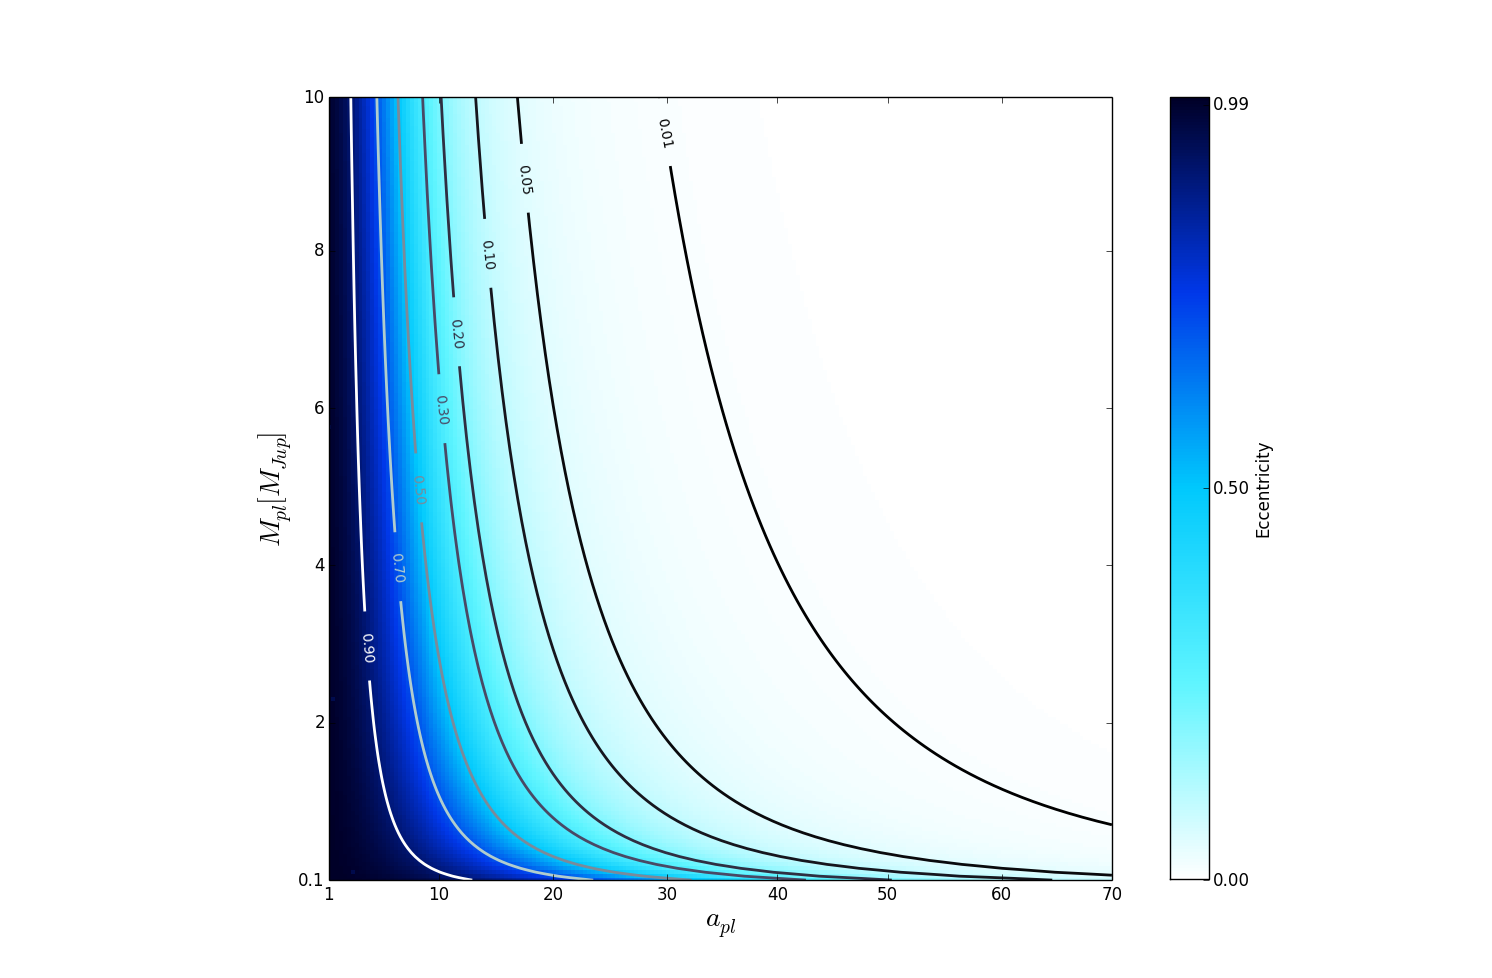
\includegraphics[width=1.6\textwidth]{49CET_stirPlot_Good_newaxes3.png}}%
	\caption{The eccentricity in $a_{pl}$, $M_{pl}$ parameter space needed to stir the planetesimal belt at $\sim$ 110\,AU in less than 49 Ceti's age of 40\,Myr. The contour lines correspond to $e_{pl}$ = 0.01, 0.05, 0.10, 0.20, 0.30, 0.50, 0.70, and 0.90.}
	\label{fig:49CET_StirringPlot}
\end{figure}

%Using Jupiter's orbital characteristics from earlier, and its mass, $M_{pl} \approx 10^{-3} M_{\odot}$, we find that the timescale for perturbing planetesimals at 110AU is on the order of 10 billion years. 

Figure \ref{fig:49CET_StirringPlot} displays the eccentricity required for a planet of semi-major axis $a_{pl}$ and mass $M_{pl}$ to stir the planetesimal belt at 110\,AU in less than 49 Ceti's age of 40\,Myr. A Jupiter-like planet, with $e_{pl}~\sim$ 0.05, $a_{pl}~\sim$ 5.2\,AU, and $M_{pl} \approx 10^{-3} M_{\odot}$, can not be responsible for stirring the ring. However, if this planet were at $a_{pl}~\sim$ 40\,AU (holding $e_{pl}$ and $M_{pl}$ constant), it would be able to excite planetesimals to collisional velocities in less than the age of the system. 

%Equation \ref{eq:planetExciteTime} is very sensitive to the eccentricity of the given planet, so 

%More realistic timescale estimates come easily from increasing the eccentricity, 

%are highly sensitive to the eccentricity. 

%Excluding the time that it takes to actually form this reference planet, 

%a more realistic timescale estimate of roughly 40Myr for the stirring of 49 Ceti's planetesimal ring is obtained if this Jupiter mass planet were at a separation of $a_{pl}$ = 40\,AU (holding everything else constant). 

%Another realistic situation is that of a 10$M_{Jup}$ planet at $a_{pl}$ = 20\,AU, which would also have a stirring timescale of $\sim$ 40Myr for the ring.

Both planetary-stirring and self-stirring are viable options for maintaining the level of collisions necessary to sustain 49 Ceti's planetesimal ring. \cite{Must09} suggest that there is a radius beyond which the disc will stir itself before a giant planet can stir it, and describe this radius as:

\begin{equation}
\label{eq:planetvself}
\Phi \sim 630~x_{m}^{-0.77} (1-e_{pl}^{2})^{-1}e_{pl}^{\sfrac{2}{3}}\bigg(\frac{a_{pl}}{1\text{AU}}\bigg)^{2}  \bigg(\frac{M_{pl}}{1M_{\odot}}\bigg)^{\sfrac{2}{3}} \bigg(\frac{M_{\bigstar}}{1M_{\odot}}\bigg)^{\sfrac{-4}{3}}~~[\text{AU}]
\end{equation}

From the opposite perspective, if a dust ring exists within the value given by Equation \ref{eq:planetvself}, it must be planet-stirred. As we showed earlier, $x_{m} \gtrsim 8$ for self-stirring to have acted out to 110\,AU within 40\,Myr. This is the one case for which 49 Ceti's planetesimal ring is self-stirred, assuming any Jupiter-like planets are within $\sim$ 40\,AU. If a planet with Jupiter's orbital characteristics exists at any separation larger than $\sim$ 40\,AU, $\Phi > 115$\,AU (holding $x_{m}$ at 8), implying that planet-stirring would be responsible for the dust ring. 

While having 8 times the ``minimum mass 49 Ceti nebula" is certainly possible, it isn't very likely. \cite{Andr13} find observationally that the median mass ratio of a protoplanetary disk to its host star is $\sim$ 0.3$\%$, that the upper quartile has $\sfrac{M_{disk}}{M_{\bigstar}} \geq 1\%$, and that only a handful have $\sfrac{M_{disk}}{M_{\bigstar}} \geq 10\%$. The MMSN is 0.013\,$M_{\odot}$\citep{Desc07}, so 49 Ceti's minimum mass nebula would have a mass of 0.026\,$M_{\odot}$. 8 times this mass gives $\sfrac{M_{disk}}{M_{\bigstar}} = 10.4\%$, which puts it just on the edge of possibility. 

If the initial mass of 49 Ceti's protoplanetary disk were closer to the median suggested by \citeauthor{Andr13}, ie. $M_{disk} = 0.006\,M_{\odot}$ and $x_{m} \sim$ 0.25, there are still many plausible scenarios in which planets are responsible for exciting planetesimals in the ring. In order for a planet to stir the ring in less time than the age of the system, it must be at a separation of at least 40\,AU from the star (with $e_{pl}~\sim$ 0.05 and $M_{pl} \approx 10^{-3}\,M_{\odot}$, as earlier) as per Equation \ref{eq:planetExciteTime}. Even if $x_{m} <$ 0.25, planetary stirring can still be responsible for stirring the ring in a timescale less than the age of the system, as $x_{m}$ affects the timeline for self-stirring but not the timeline for planet stirring. $x_m$ likely has a significant influence on the timescale for giant planet formation, but this connection is not well established and is only starting to be probed with observations. 

%Based on this analysis, it is more likely that a planet between 1-10$M_{Jup}$ at a separation greater than 40AU (for the 1$M_{Jup}$ planet) or 20 AU (for the 10$M_{Jup}$ case) is responsible for stirring the planetesimal ring. These planets need to coalesce quickly enough such that their gravitational impact on the ring occurs in less time than the combined age of their formation and timescale of influence, so it is probable that the previous estimates of mass and semi-major axis for a perturbing planet are on the low end, as these hypothetical planets would take the full 40Myr of 49 Ceti's lifetime to stir the ring. 

For example, recent evidence of planet formation in the 1-2\,Myr old HL Tau system \citep{Part15} suggests these processes may happen much more quickly than in the canonical outlook, which says that giant planets must form within $\sim$ 10\,Myr of stellar formation \citep{Poll96}. Estimates of the dust mass in HL Tau's disk range between 0.03-0.14\,$M_{\odot}$ \citep{Robi07}, which relative to its stellar mass of 0.7\,$M_{\odot}$ \citep{Clos97} suggest $x_{m} \gtrsim$ 3-16 (remember $x_{m}$ = 1 corresponds to when $M_{disk}$ = 0.013\,$M_{\bigstar}$). HL Tau's disk displays ring-like structure in alternating light and dark bands out to $\sim$ 100\,AU, with the spectral index of the darker rings suggesting significant grain growth. Large planets have probably coalesced and are responsible for shaping these gaps in the disk.

%a series of light and dark rings at wavelengths between 870$\mu m$ and 2900$\mu m$, %With such a massive protoplanetary disk, it is apparent that planet forming processes occur rapidly. 

HL Tau shows us that large values of $x_{m}$ leads to planet formation processes out to $\sim$ 100\,AU in short timescales, providing additional circumstantial evidence that 49 Ceti's ring may be planet stirred. If $x_{m}$ were large enough such that self-stirring could be viable, it is likely that giant planets would form beyond a critical $a_{pl}$ that sets the critical radius $\Phi$ for which a ring would be planet stirred or self stirred for a given $x_{m}$ (Equation \ref{eq:planetvself}). If $x_{m}$ = 8 (the minimum for a self-stirring scenario for 49 Ceti's ring), it is logical, as per observations of HL Tau, that giant planets would be forming throughout the disk in only a few Myr. In this situation, any planet slightly more massive, closer, or more eccentric than that suggested by Figure \ref{fig:49CET_StirringPlot} (as to leave a few Myr for planet formation) would be responsible for the stirring. 
%Leaving a few Myr for formation of the planet, any planet with a suitable combination of $M_{pl}$, $a_{pl}$, and $e_{pl}$ as described by Figure \ref{fig:49CET_StirringPlot} would 
%Based on the timescales for planetary stirring suggested by Equation \ref{eq:planetExciteTime} and the critical radius from Equation \ref{eq:planetvself}, planets slightly larger or closer than the 10$M_{Jup}$ planet at 20AU and 1$M_{Jup}$ planet at 40AU (larger or closer such that stirring timescales would be shorter, leaving a few Myr for formation) would be responsible for the stirring. 

If the planetary stirring scenario is indeed the correct one, this has significant implications for planet formation. \cite{Must09} posit that the largest planetesimal that an interior planet can destroy at a separation $a$ is given by:

\begin{equation}
\label{eq:planetDestruction}
R_{max} \approx 74 \bigg(\frac{e_{pl}}{0.1}\bigg) \bigg(\frac{M_{\bigstar}}{M_{\odot}}\bigg)^{\sfrac{1}{2}} \bigg(\frac{a}{10\text{AU}}\bigg)^{\sfrac{-3}{2}} \bigg(\frac{a_{pl}}{1\text{AU}}\bigg)~~[\text{km}]
\end{equation}

The 1\,$M_{Jup}$ planet at 40\,AU considered earlier would be able to destroy planetesimals up to radii of $\sim$ 50\,km at 110\,AU and $\sim$ 200\,km at 50\,AU. This suggests that growth of planetesimals beyond this barrier would become extremely difficult after the aforementioned planet coalesced. Even if bodies larger than this existed prior to the this planet's formation, the resulting increase in the velocity dispersion from the Jupiter-mass planet would impede growth rates. This suggests that multiple planet systems form simultaneously, as there are significant disturbances in the disk after large planets have formed. 

%Note that Equation \ref{eq:planetDestruction} is not dependent on the mass of the planet, but rather is linear with respect to the planet's eccentricity and semi-major axis. 

\subsection{Broad Dust Disk Component}

From our modeling, we find that 49 Ceti's outer disk beyond the surface density enhancement at $\sim$ 110\,AU is well described by a decreasing power law, with $\Sigma \propto r^{-0.8}$ for the USDE model and $\Sigma \propto r^{-1.5}$ for the double power law. The standard point of comparison for disks is the surface density of the MMSN \citep{Weid77,Haya81}, which is found to fall off as $r^{-1.5}$ (see Equation \ref{eq:MMSNsurf}). However, this assumes that the planets of the Solar System formed in situ. If the planets have undergone significant radial migration, which is certainly possible \citep{Levi03}, the inferred density profile for the MMSN could be significantly distorted from the true initial conditions. Observations of 24 circumstellar disks in the $\sim$ 1\,Myr old Ophiuchus-Scorpius and Taurus-Auriga star forming region find that $\Sigma \propto r^{-1}$ after the removal of systematic effects \citep{Andr07}, and subsequent analysis of the nine brightest protoplanetary disks in Ophiuchus corroborate this result, finding that the median initial surface density falls off as $r^{-0.9}$ \citep{Andr09}.  

In 40 million years of evolution, however, it is logical to expect that the processes shaping the disk should have altered it significantly from initial conditions. Steady accretion disks, with $\alpha$ constant and the viscosity proportional to the radius, have $\Sigma \propto r^{-1}$ \citep{Shak73,Hart98}. In addition, simple mass conservation arguments for a disk where radiation pressure driven outflows dominate show that the surface density should fall off as $r^{-1}$, which matches the profile of Vega's debris disk \citep{Su05}. 

Rings of increased collisions of planetesimals, which generate a large diversity of grain sizes, can have a distinct impact on the morphology of the rest of the disk. One such ``birth ring," in AU Mic, acts as the divider between an inner disk of millimeter-sized grains and an outer disk of micron-sized grains. \cite{Stru06} suggest that the small grains migrate outwards due to radiation pressure, whereas large grains fall inward due to corpuscular and Poynting-Robertson (CPR) drag. Further, they show that the outer disk is collision-dominated, as the population of small grains falls off as $r^{-3/2}$, matching theory. 

The hypotheses put forth to explain the distribution of grains in the case of Vega and AU Mic only describe the expected surface density profile of micron-sized grains and do not touch on the processes that shape millimeter-sized grains in debris disks. It is tempting to extend the theories that describe the small grains to larger grains, but the morphology of micron-sized grains can be different from the larger grains traced by our observations. Using conjectures for the processes that shaped these disks to describe 49 Ceti's disk, which seems to show the opposite arrangement of small and large grains, would be unwise. Although collisions, radiation pressure, and CPR drag certainly play a role in sculpting 49 Ceti's dust disk, the presence of gas complicates how these mechanisms act. More theoretical modeling is needed before we will be able to understand the processes responsible for different surface density profiles of millimeter grains.  

%The evolution of debris disks, whether gas-poor or gas-rich, is not well understood, 


%However, this argument considers grains just above the blowout size (i.e. $\sim$ 10$\mu m$), and the morphology of these grains can be different than the larger grains traced by our observations. 


%, and that this power law describes the scattered light images of AU Mic well. 



%find AU Mic's outer disk of small grains is collision-dominated, as it lined up with predictions showing that small grains should fall off as $r^{-3/2}$ in this case. 

%In collision-dominated disks, the outer population of small grains should fall off as $r^{-3/2}$ \citep{Stru06}, and this is four to 

%This phenomenon is observed in AU Mic, where grains of all sizes are created in one of these rings $\sim$ 40AU from the star. 

%Beyond this ring, only micron-sized grains are observed, whereas millimeter-sized grains are seen in the inner disk \citep{Macg13}. The surface density distribution of the outer disk is sensitive to what processes dominate. If corpuscular and Poynting-Robertson drag dominate, the distribution of micron sized grains should fall off as $r^{-5/2}$, whereas the population of grains in collision-dominated disks falls off as $r^{-3/2}$ \citep{Stru06}. 

% due to processes that act differently on each grain population. 


%$In addition, certain accretion disk collapse scenarios predict $\Sigma \propro r^{-1}$ \citep{Shak73}. 

%http://iopscience.iop.org/0004-637X/632/1/670/pdf/62699.web.pdf

%, with relatively gentle power law slope, 

%-0.8pm0.2 for bBBAG
%-1.3pm0.1 for nOBAG
%-1.5pm0.2 for dPBAG


\section{Gas Disk Characteristics}

\begin{figure}
\centering
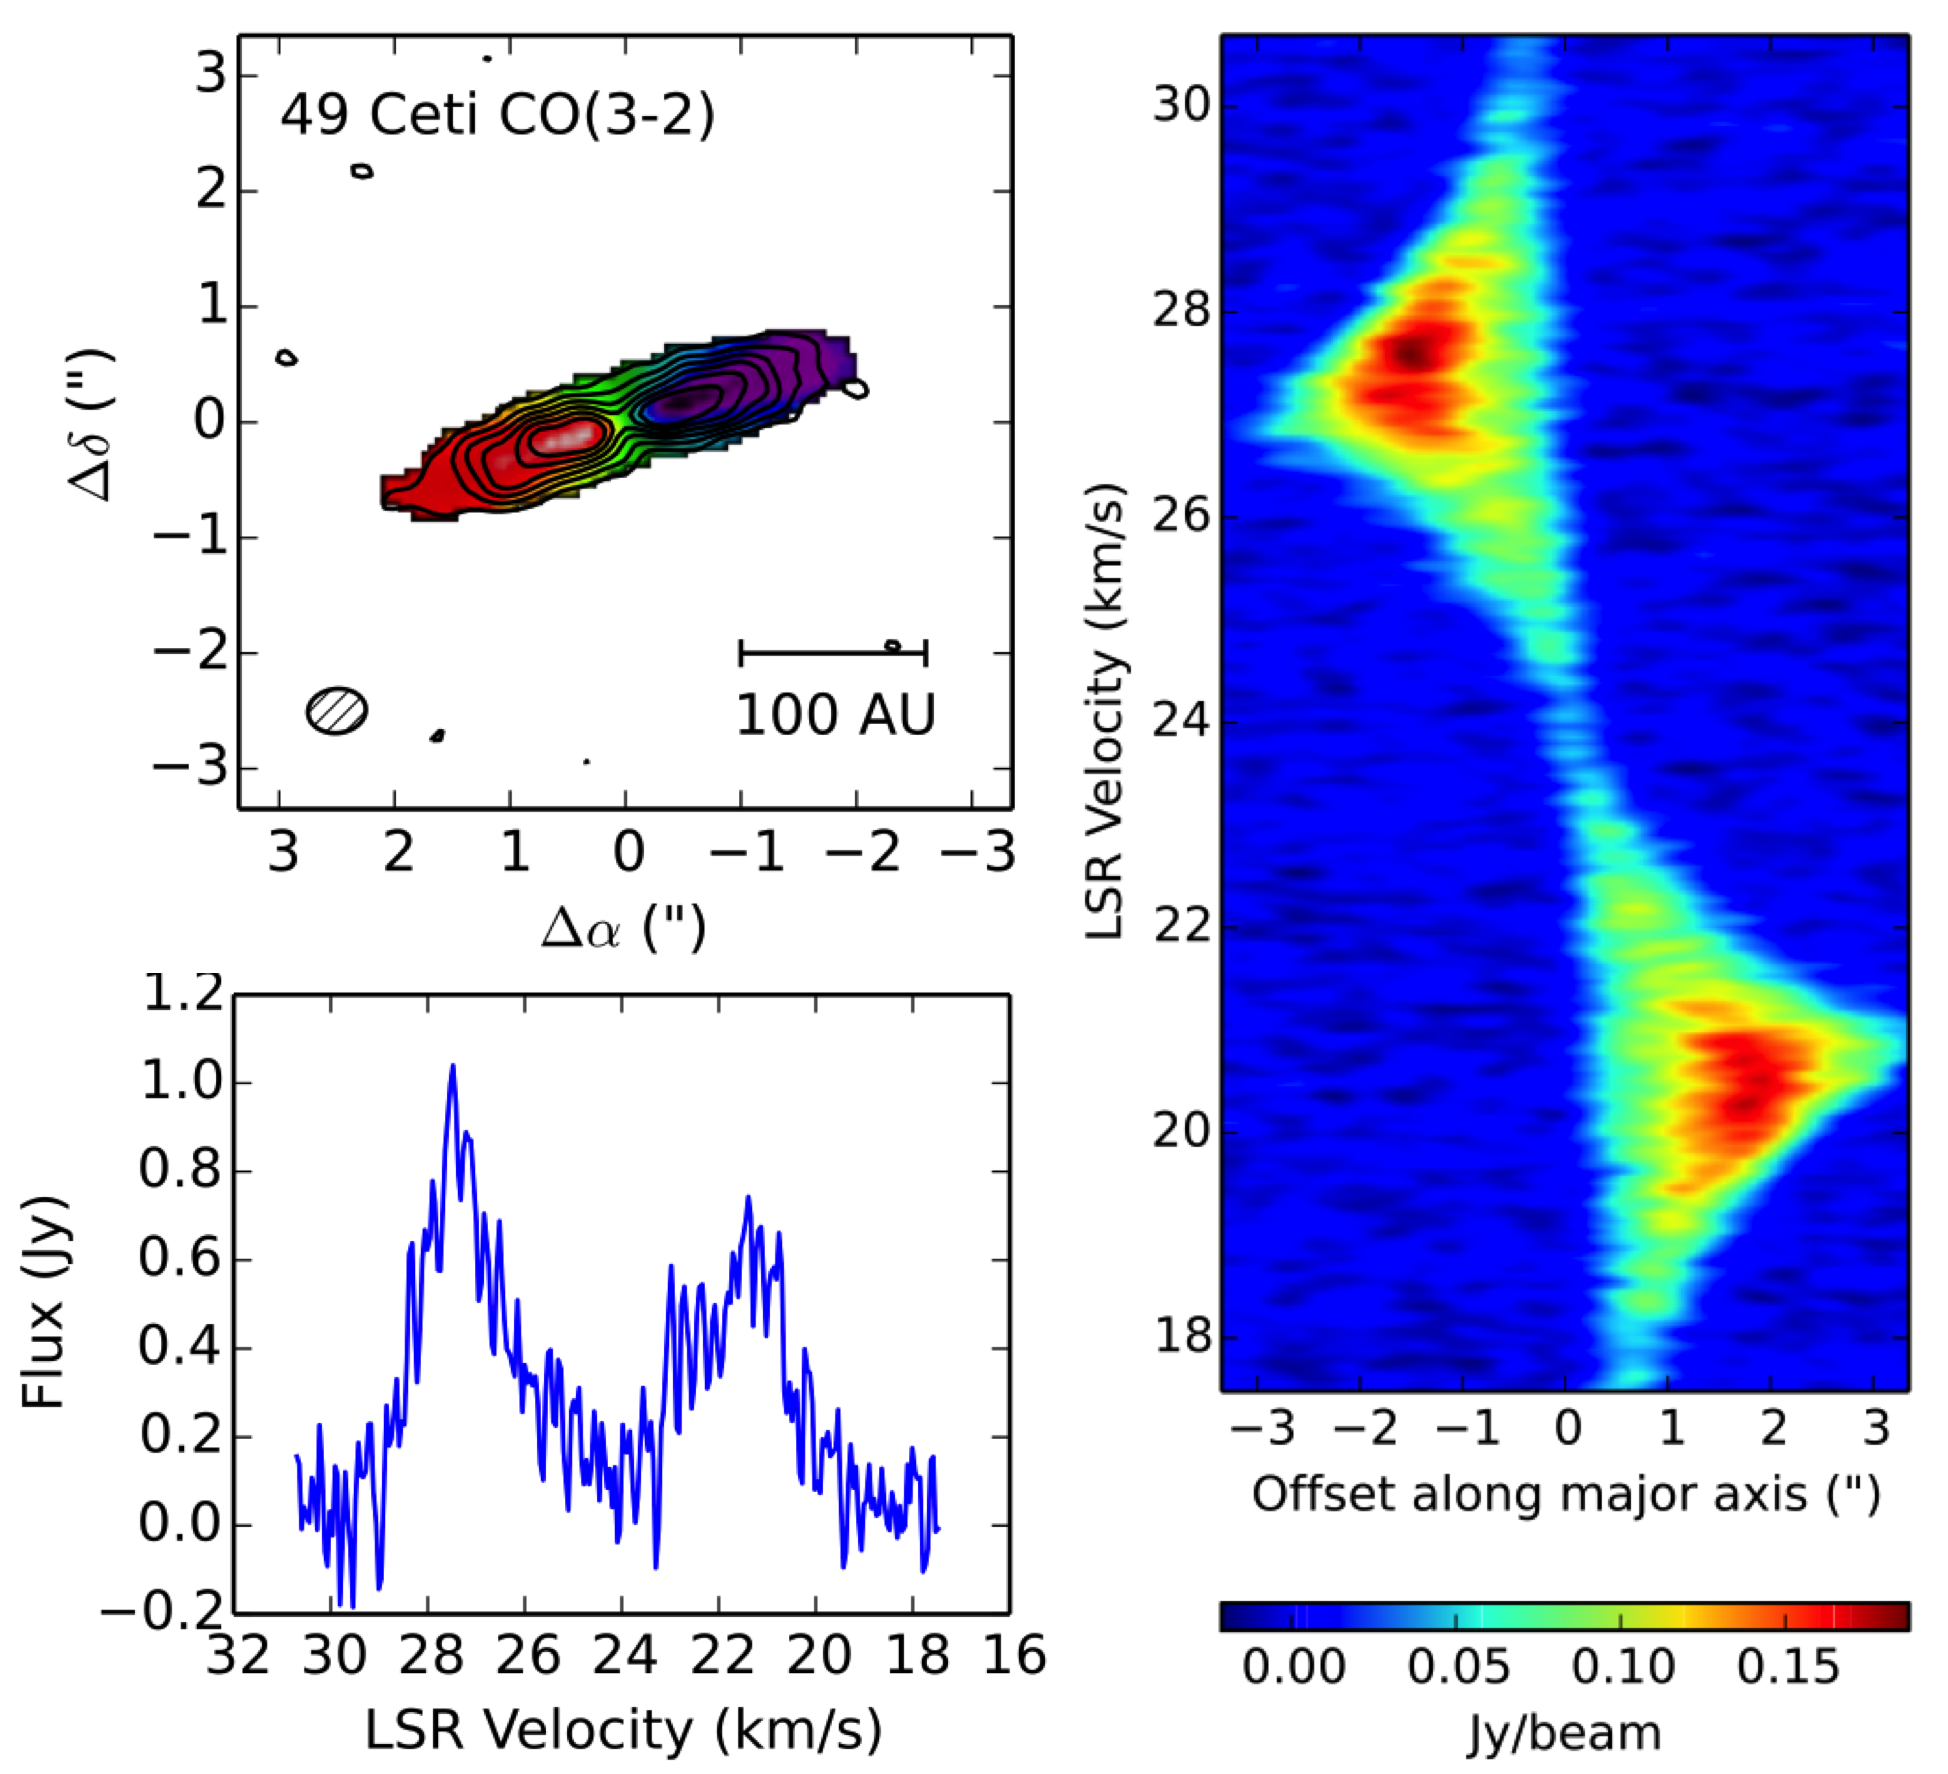
\includegraphics[width=\textwidth,height=\textheight,keepaspectratio]{49CET_CO_plots_sideby.png}
\caption{The zeroth (contours) and first (colors) moment maps are displayed in the top left panel. The contours are [3, 6, 9, 12, 15, 18] $\times$ 0.02 Jy beam$^{-1}$. The CO(3-2) spectrum is shown in the bottom left. The line exhibits a double-peaked structure that is characteristic of an inclined disk in Keplerian rotation about the central star. The southeast side of the disk is $\sim 40 \%$ brighter in integrated emission than the northwest side. A position-velocity diagram of CO(3-2) emission from the gas disk is presented in the right panel. The x-axis represents offset position from the southeast limb to the northwest limb along the disk major axis relative to the star position.}
\label{fig:49CET_CO_plots}
\end{figure}

Modeling of the CO detected around 49 Ceti at the J=3-2 transition has been inconclusive thus far. However, examination of the zeroth moment map and position-velocity (PV) diagram (see Figure \ref{fig:49CET_CO_plots}) reveals basic characteristics of the gas morphology. A separation of 1.43 $\pm$ 0.03 arcsec exists between the two peaks apparent in the zeroth moment map, corresponding to a separation of 87\,AU. This, in combination with the lack of a central peak and the relatively faint line emission indicating that the gas is optically thin, suggests that the inner disk is gas-poor within 44\,AU. This value is probably underestimated, however, as the beam detects flux from the front and back of the disk along the minor axis due to the disk's high inclination. This inner radius is consistent with the value of $\sim$ 90\,AU derived from CO(2-1) observations performed \cite{Hugh08} with the SMA. At its maximum along the major axis, 3$\sigma$ emission extends 7.3 $\pm$ 0.1 arcsec, which suggests the outer radius of the gas disk is $\sim$ 220\,AU. 

Preliminary models of the gas disk indicate $\sim 7 \times 10^{-7} M_{\odot}$ of CO (assuming a CO/H$_{2}$ abundance of 10$^{-4}$), and seem to show an increase in the density of gas at $\sim$ 100\,AU. The peak of nearly 0.20\,Jy\,beam$^{-1}$ in the PV diagram on the southeast side of the disk is separated by $\sim$ 1.6'' ($\sim$ 100\,AU) from the star's position, corroborating the results of those early models. While it appears that the southeast side of the disk is brighter in the spectrum and the PV diagram, this difference is not significant. 

\section{Gas in Debris Disks}

49 Ceti's three part dust disk, consisting of an inner disk of small grains and a broad outer disk of larger grains punctuated by a surface density enhancement, is unlike all other debris disk that have been studied in this level of detail. This, in combination with its significant mass of gas given its age, make it truly unique. However, there are a handful of other systems that seem like siblings to 49 Ceti---they are clearly all related, but none of them look quite the same. 

The gas we observe in other gas-rich debris disks can be primordial, left over from the formation of the star, or secondary, released through collisions of planetesimals. Protoplanetary disks are good at nursing large masses of gas due to effective shielding from the optically thick dust content \citep{Wyat14}, but as the dust disperses, the rate of photodissociation of gas accelerates, and most disks are found to be gas-poor by an age of 10\,Myr \citep{Zuck95}. In systems that display co-located gas and dust, the gas is assumed to be continually replenished by the same collisional mechanisms responsible for sustaining the secondary dust content, but in systems that display distinct gas and dust disks, another explanation is needed for explaining the presence of gas. Assuming the composition of comets and other icy bodies in exoplanetary systems is similar to that in the solar system, i.e. $\sim$ 10$\%$ CO by mass, maintaining the gas disk requires a hearty but not unreasonably large diet of volatile-rich dust, planetesimals, and comets. 

\subsection{ALMA-Resolved Gaseous Debris Disks}

In addition to 49 Ceti, the only gas-rich debris disks to be imaged in both gas and dust emission with ALMA are $\beta$ Pic and HD 21997. These systems provide a timeline for us to examine the processes that are shaping the gas and dust at this late stage of disk evolution. However, each displays distinct characteristics, exemplifying that this picture is not a simple one.

$\beta$ Pic, an A star, hosts a gaseous debris disk viewed edge-on that is very similar to 49 Ceti's. At only 19\,pc away, it was one of the first of its kind to be discovered and has been studied extensively both with resolved millimeter observations (with the SMA by \citealt{Wiln11}, ALMA by \citealt{Dent14}) and in coronographic scattered light imaging (first by \citealt{Smit84}, with STIS by \citealt{Heap00}, more recently by \citealt{Ahmi09}, \citealt{Mill14}, and \citealt{Apai15}). Its disk has a dust mass of $\sim 8\times10^{-2}$ $M_{\oplus}$ and $\sim 4\times10^{-5}$\,$M_{\oplus}$ of CO \citep{Dent14} at an age of $\sim$ 20\,Myr \citep{Bink14}. The millimeter dust probed by ALMA is distributed in an azimuthally asymmetric belt that is nearly co-located with sub-microns grains that have been revealed in scattered light imaging. The surface brightness peaks at 60\,AU from the star, nearly matching the inner radius of the gas disk, which extends from 50 to 160\,AU, peaking at 85\,AU. The CO dissociation timescale in $\beta$ Pic's outer disk is on the order of 100 years because of ionizing interstellar radiation, so CO is either continually replenished or we are observing the system $<$ 100 years after a significant collision. \cite{Moor15} found that given $\beta$ Pic's outer radius, a planet-stirring scenario is probably responsible for spurring collisions within the disk. 

%$12^{+8}_{-4}$ Myr \citep{Zuck01}.

%The birth ring at $\sim$ 40AU is likely creating grains of all sizes that are subject to different 

%reveal strong forward scattering and polarization out to $\sim$ 80AU, and the specifics arounhinting that the birth ring is made of highly porous ($\sim 90 \%$) primordial ices that formed beyond the frost line \citep{Grah07}. 

%resolved by SMA \citep{Wiln12}
%ACS on HST -- first polarization maps!! find that grains must be highly porous ($\sim90\%$)... possibly primordial because the birth ring lies beyond ice sublimation point \citep{Grah07}
%scattered light by \citep{Kala04}, \citep{Kris05}

The 30\,Myr old A star HD 21997, 72\,pc away, also hosts a gaseous debris disk. The dust disk extends from 55 to 150\,AU with the surface density decreasing as $\sim r^{-1.6}$ and has a mass of $\sim 9\times10^{-2}$\,$M_{\oplus}$ \citep{Moor13}. An estimated $\sim 6\times10^{-2}$\,$M_{\oplus}$ of CO extends from $\sim 25$\,AU to  $\sim 140$\,AU \citep{Kosp13}. The dust and gas seem to be co-located between 55 and 140\,AU, but within 55\,AU is a dust-poor inner region. 

The distinct locations of the dust and gas populations hint that different processes may be shaping their morphologies. \cite{Kosp13} suggest that the CO is primordial and has endured since the formation of the star due to very efficient shielding mechanisms, as maintaining the observed mass of CO through collisions of planetesimals and comets would require an unreasonably high gas production rate of 10$^{19}$\,kg\,yr$^{-1}$ ($\sim 10^{-6}\,M_{\odot}$\,yr$^{-1}$). However, \cite{Moor13} posit that the dust is secondary, as models by \cite{Kriv09} state that the lifetime of grains in a gaseous debris disk with a gas-to-dust ratio of 100 is less than 2 $\times$ 10^{4} years. As with $\beta$ Pic, HD 21997's disk is probably planet stirred, as its outer radius is greater than a 10 minimum mass stellar nebula could self-stir to within 30\,Myr \citep{Moor15}. If correct, the primordial gas scenario implies efficient radial drift of grains due to strong gas-dust coupling, which hints that the extended dust disk could be the result of efficient migration from a narrow, planet-stirred planetesimal ring. 

HD 141569, an A star $\sim$ 110\,pc away that is 5\,Myr old, displays CO emission in addition to displaying the qualities of a debris disk, but the gas disk has not yet been resolved with any millimeter interferometer. Scattered light imaging by \cite{Wein00} reveals that the disk extends out to $\sim$ 360\,AU with a gap in the disk at $\sim$ 250\,AU. Gaps like these are suggestive of continual clearing and secondary dust production processes. \cite{Brit07} find that the gas emission comes from within $\sim$ 40\,AU of the star, but it is unclear if the dust traces the gas, as the scattered light imaging is only able to see micron-sized grains at greater than $\sim$ 70\,AU and millimeter observations have not been performed. 
%This extreme pace, equivalent to the complete destruction of $\sim$ 6000 Hale-Bopp sized comets each year, argues against the secondary replenishment scenario, unless we are observing HD 21997

%HD 21997's disk has not been detected in scattered light by recent \textit{HST} observations \citep{Kris10}, implying a low albedo for the grain population. However, this non-detection could also result from the disk falling below the sensitivity limit of the ACS coronagraph due to the distance of the system. 

\section{Debris Disks Resolved by ALMA}

The resolution and sensitivity now available with ALMA in examining continuum emission from circumstellar material is helping detail how secondary dust is created and the processes that shape its morphology. Often, the dust is produced in a ``birth ring," which has an enhanced region of collisions relative to other parts of the disk. The handiwork of planets can appear as distinct structures of the surface density. Clearing by a planet can result in a distinct gap in the dust disk, whereas a narrow ring with abrupt cutoffs suggests gravitational interaction with one or more planets.

%The of this birth ring has implications for the timescale since stirring began, as the spread of grains in opposite directions by forces that work differently on small and large grains. 

The M-type star AU Mic, part of the $\beta$ Pic moving group at an age of $\sim$ 20\,Myr, hosts an edge-on debris disk that displays no CO emission. As with $\beta$ Pic, its proximity to Earth (10\,pc) has made it a popular target for observation. Millimeter observations with the SMA by \cite{Wiln12} and with ALMA by \cite{Macg13} find that the dust disk increases steeply in surface density ($\Sigma \propto r^{2.3}$) from $\sim$ 10-40\,AU before abruptly dropping off. This profile can be explained by a self-stirred disk with ongoing planet formation \citep{Kenn10}, but the timescale required to initiate the collisional cascade is much longer than its age (as per Equation \ref{eq:t1000km}, \citealt{Keny08}). Thus, planetary stirring is the likely cause of the peak in surface density at $\sim$ 40\,AU. Scattered light imaging detects the disk out to $\sim$ 210\,AU \citep{Kala04,Kris05}, and models of polarization maps of the disk indicate micron-sized grains extend from $\sim$ 40\,AU to $\sim$ 150\,AU \citep{Grah07}. \cite{Stru06} suggest that a birth ring exists at $\sim$ 40\,AU in which grains of all sizes are created through collisions. The smaller grains, highly susceptible to stellar winds and radiation pressure, are blown out on highly eccentric orbits, whereas larger grains fall inward due to CPR drag. 

The 100\,Myr G-type star HD 107146 and its gas-poor disk give a snapshot of the very late stages of debris disk evolution. At 28\,pc, it has been resolved at millimeter wavelengths with CARMA \citep{Cord09} and the SMA \citep{Hugh11}, but recent Cycle 0 observations with ALMA are able to ascertain more detailed structure \citep{Ricc15}. The ALMA continuum data detect emission from 30-150\,AU that can be equivalently modeled by a double power-law for the surface density that decreases to $\sim$ 70\,AU before increasing thereafter and by a shallowly increasing single power-law with a $\sim$ 8\,AU gap at $\sim$ 80\,AU. The simplest explanation for the clearing in the dust disk is that a planet of a few $M_{\oplus}$ has coalesced and cleared a nearly circular orbit at $\sim$ 80\,AU. The increasing surface density in the outer disk can be explained by a self-stirring scenario, but only if $x_{m} \geq 10$, which is unlikely but not impossible (see Section \ref{SelfStirring}). 

Optical and near-IR scattered light imaging of HD 107146 revealed micron sized grains extending from $\sim$ 50 to $\sim$ 230\,AU, with a peak in density at $\sim$ 130\,AU \citep{Ardi04,Erte11}. Like in $\beta$ Pic, where micron-sized grains are not co-located with their larger brethren, the two grain populations in HD 107146 show distinctly different morphologies. This isn't necessarily unsurprising, as grains in HD 107146's disk have been subject to the physical mechanisms of CPR drag and radiation pressure that act more efficiently on small grains for longer timescales. 

At $\sim$ 440\,Myr old and only $\sim$ 8\,pc away, the debris ring around the A star Fomalhaut is one of the oldest that has been thoroughly studied. Early efforts to observe the ring at millimeter wavelengths \citep{Holl98,Ricc12} detected the ring but lacked the resolution to accurately trace the emitting grain population (and thus the parent body morphology). However, more recent ALMA observations resolve the eccentric ring and find it is $\sim$ 15\,AU wide with sharp inner and outer boundaries, has a semi-major axis of $\sim$ 140\,AU, and has an eccentricity of $\sim$ 0.1 \citep{Bole12}. These observations are in agreement with scattered light imaging by \cite{Kala05} that showed a peak brightness in scattered optical light at the same distance. The morphology of the ring suggests that it is confined by gravitational interaction with one or more planets \citep{Chia09}.

\section{49 Ceti in Context}

49 Ceti is a rare example of a gas-rich debris disk, displaying properties not observed in protoplanetary disks. The broad dust disk characterized by two grain sizes underlying the enhancement at $\sim$ 110\,AU is a unique morphology that hasn't been observed in other systems. Although the inner disk doesn't necessarily fill out all the way to $R_{Inner Disk}$ (this was an assumption in modeling following the approach of \citealt{Wahh07}), there is a clear transition at this radius where an outer disk of larger grains begins. The mechanisms responsible for distinct populations of small ($\sim 0.1 \mu m$) grains in the inner disk and larger ($\sim 1.6 \mu m$) grains in the outer disk is not well understood given our data. We hypothesize that the dust in 49 Ceti's planetesimal ring at $\sim$ 110\,AU is continually replenished and that it is probably stirred by an interior planet (Section \ref{PlanetStirring}). 

\begin{figure}
	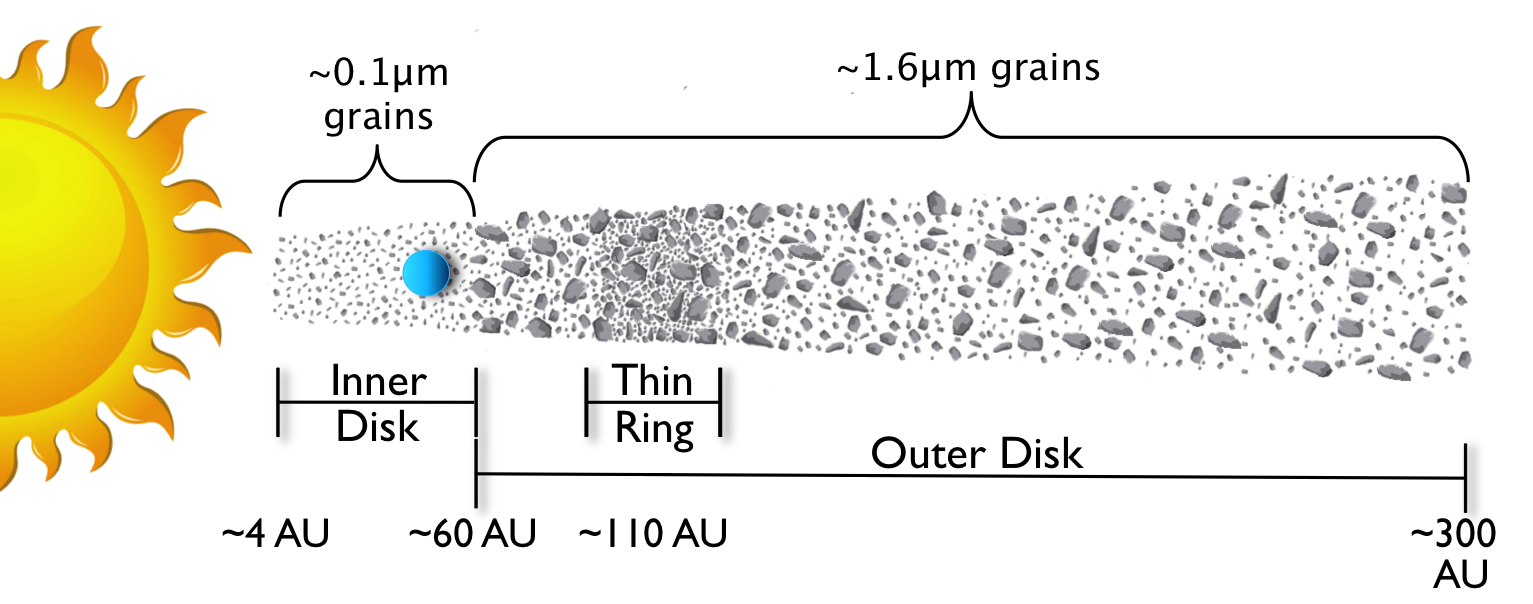
\includegraphics[width = 1\textwidth]{49CET_DustDistributionCartoon2_ForThesis.png}
	\caption{A cartoon of the dust distribution of 49 Ceti. The enhancement in the surface density is shown as a narrow ring here (the USDE model, see Section \ref{USDE}), but it can be equivalently described by a double power law that peaks at this radius (see Section \ref{DP}). We find that planetary stirring is responsible for promoting collisions in this planetesimal belt, but our data are unable to constrain the location or mass of this planet.}
	\label{fig:49CET_DDC}
\end{figure}

The diversity of debris structures that have been previously observed exemplify how complex disk evolution is and 49 Ceti only adds to this intricate picture. The sharply increasing surface density structure of AU Mic is consistent with predictions for self-stirring, but the 1000-km planetesimals at the peak density of the ring necessary for this scenario could not have in the age of the system, suggesting planetary stirring may be responsible. However, no gaps in the surface density distribution suggestive of planets, such as the one in HD 107146, are observed in AU Mic. Fomalhaut's ring seems more typical of older debris systems that have had more time to evolve. Of the gas-rich debris disks, HD 21997 shows a dust disk with a steeply decreasing power law for the surface density that doesn't seem to be co-spatial with the gas disk, whereas $\beta$ Pic's gas and dust disks are effectively co-located. 49 Ceti's dust disk, with a peak in the surface density on top of a broad decreasing component, doesn't resemble any of the debris disks with no gas or HD 21997, but it's disk is quite similar to $\beta$ Pic's disk.
%; additionally it helps to limit the number of parameters needed to recreate the data

Preliminary analysis puts a strong lower limit for the inner edge of the 49 Ceti's gas disk at 44\,AU and suggests a peak in the density at $\sim$ 100\,AU, which corresponds closely with the geometry of the outer dust disk. This co-location of material signifies that secondary processes are almost certainly responsible for producing the gas and dust we observe at this late stage of disk evolution. $\beta$ Pic displays essentially this same structure, although the distribution of small grains is slightly different in these two systems. For 49 Ceti, small grains are limited to an inner disk that extends roughly $\sim$ 60\,AU from the star \citep{Wahh07}, whereas in $\beta$ Pic, small grains permeate through the entirety of the outer disk of millimeter grains as resolved by ALMA \citep{Apai15}. In addition, 49 Ceti displays no brightness asymmetry in CO or dust emission, though $\beta$ Pic does. As asymmetries in debris rings can arise easily from 2:1 mean-motion resonances with inner planets, this suggests the birth ring of $\beta$ Pic may be at roughly twice the radius of an unseen interior planet of $>10~M_{\oplus}$ \citep{Dent14}. The lack of an asymmetry in 49 Ceti's planetesimal belt could mean that the giant planet responsible for stirring isn't in resonance with the ring, or that our observations aren't high enough sensitivity to detect any asymmetry.






%T%his morphology, as is true in $\beta$ Pic as well, suggests 
%This may signify that similar processes are shaping the gas and dust disks at this late stage of disk evolution. As the ages of 49 Ceti, $\beta$ Pic, and HD 21997 are older than the timescale during which gas and dust generally disperse and few efficient shielding mechanisms are apparent, it is likely that the dust and CO that we observe is second-generation, produced through collisions of planetesimals and icy bodies. 

%, this would mean 49 Ceti is similar to $\beta$ Pic. This likely asymmetry raises the possibility of a $>10~M_{\oplus}$ planet in the outer disk that shepherds the dust and gas in a mean-motion resonance, increasing the likelihood of collisions at a specific radius, as may be the case in $\beta$ Pic (Dent et al.\ 2014). This would help explain how such a significant mass of co-located CO and sub-mm dust continue to be visible as 49 Ceti ages. 


%Generally it is expected that disks with actively stirred planetesimal rings have similar morphologies (optical vs mm), as collisional processes produce grains of all sizes that emit or reflect light from the optical out to millimeter wavelengths
%long wavelength images trace best the location and distribution of larger colliding bodies as the small grains probed at optical and near IR wavelengths react strongly to stellar radiation and wind forces... large grains in mm emission have dynamics like parent planetesimals (not my words) \citep{WYATT2006 IF YOU USE THIS, see sec. 6 of 107146 paper}. 

%CO is not detected, suggesting that the primordial gas has dispersed or coalesced into large bodies and that it is not being replenished. 


%The typical size of bodies in the disk affects how efficient a planet can be at promoting grinding collisions. For bodies $\sim$ 80m in size, a planet can stir the disk out to a radius given by: 
%\begin{equation}
%a = 1800\text{AU} e_{pl}^{\sfrac{2}{3}} \bigg(\frac{M_{\bigstar}}{1M_{\odot}}\bigg)^{\sfrac{1}{3}} \bigg(\frac{a_{pl}}{1\text{AU}}\bigg)^{\sfrac{2}{3}}
%\end{equation}

%MARS SIZED COLLISION???!?
%rare. talk beta pic and its asymmetry. 



%Observations at sub-millimeter wavelengths trace emission from large, $>100\mu m$ grains. Gas free-- little affected by radiative forces-- gas weak-- only weak coupling between gas and dust (TAKEUCHI & ARTYMOWICZ 2001). 

%comets sublimate at 110K (Wyatt 2008, the textbook one), so contribution of cometary gas to disk must be through collisions to be released


 %and as gas and dust lifetimes are very short 

%The co-location of gas and dust indicates that similar processes may be 


%either due to a mean-motion resonance with a giant planet or from the recent collision of mars-sized bodies
